\begin{figure}[H]
    \centering
    \begin{subfigure}{0.4\textwidth}
        \centering
        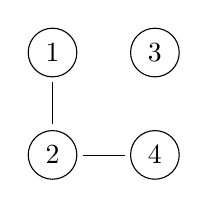
\begin{tikzpicture}[scale=1, every node/.style={circle,draw,minimum size=5mm}]
            \node (n0) at (0,1.3) {1};
            \node (n1) at (0,0) {2};
            \node (n2) at (1.3,1.3) {3};
            \node (n3) at (1.3,0) {4};
            \draw[very thin, black] (0,0.39) -- (0,0.92);
            \draw[very thin, black] (0,0.39) -- (0,0.92);
            \draw[very thin, black] (0.39,0) -- (0.92,0);
        \end{tikzpicture}
        \caption{Graf niespójny.}
        \label{fig:connected_and_not_connected_graph_a}
    \end{subfigure}
    \begin{subfigure}{0.4\textwidth}
        \centering
        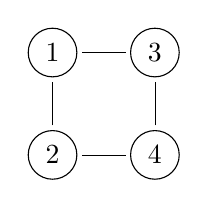
\begin{tikzpicture}[scale=1, every node/.style={circle,draw,minimum size=5mm}]
            \node (n0) at (0,1.3) {1};
            \node (n1) at (0,0) {2};
            \node (n2) at (1.3,1.3) {3};
            \node (n3) at (1.3,0) {4};
            \draw[very thin, black] (0,0.375) -- (0,0.93);
            \draw[very thin, black] (1.3,0.375) -- (1.3,0.93);
            \draw[very thin, black] (0.375,0) -- (0.93,0);
            \draw[very thin, black] (0.375,1.3) -- (0.93,1.3);
        \end{tikzpicture}
        \caption{Graf spójny.}
        \label{fig:connected_and_not_connected_graph_b}
    \end{subfigure}
    \caption{Przykłady grafów spójnych i niespójnych.}
    \label{fig:connected_and_not_connected_graph}
\end{figure}